% ============================================================================
%   Comprehensive Research Report on the GUDS-EDL Architecture
%   Mathematical Foundations, Multi-Agent Dynamics, and Clinical Applications
%
%   File: guds_edl_report_en.tex
%   Version: 2.0 (Updated 06/2026)
%   Language: English
% ============================================================================

\documentclass[letterpaper]{article} % DO NOT CHANGE THIS
\usepackage{aaai}  % DO NOT CHANGE THIS
\usepackage{times}  % DO NOT CHANGE THIS
\usepackage{helvet}  % DO NOT CHANGE THIS
\usepackage{courier}  % DO NOT CHANGE THIS
\usepackage[hyphens]{url}  % DO NOT CHANGE THIS
\usepackage{graphicx} % DO NOT CHANGE THIS
\urlstyle{rm} % DO NOT CHANGE THIS
\def\UrlFont{\rm}  % DO NOT CHANGE THIS
\frenchspacing  % DO NOT CHANGE THIS
\setlength{\pdfpagewidth}{8.5in} % DO NOT CHANGE THIS
\setlength{\pdfpageheight}{11in}
\setcounter{secnumdepth}{2}
%%%%%%%%%%
% PDFINFO for PDFLATEX
\pdfinfo{
/Title (GUDS-EDL: Uncertainty-Guided 2:4 Dynamic Sparse Evidential Learning for Extreme Imbalanced Classification)
/Author (Anonymous Authors)
}
%%%%%%%%%%
 % DO NOT CHANGE THIS

% --- Additional Packages ---
\usepackage[utf8]{inputenc}
\usepackage[english]{babel}
\usepackage{amsmath, amssymb, amsthm, bm}
\usepackage{booktabs}
\usepackage{multirow}
\usepackage{array}
\usepackage{adjustbox}
\usepackage{placeins}
\usepackage{stfloats}
\usepackage{float}
\usepackage{algorithm}
\usepackage{algorithmic}
\usepackage{enumitem}
\usepackage{tikz}
\usetikzlibrary{arrows.meta, positioning, calc}
\usepackage[table]{xcolor}
\usepackage{colortbl}
\usepackage[colorlinks=true,linkcolor=black,citecolor=blue,urlcolor=blue]{hyperref}

\newcolumntype{C}{>{\centering\arraybackslash}c}

% --- Custom commands ---
\newcommand{\Dir}{\text{Dir}}
\newcommand{\KL}{\text{KL}}
\newcommand{\R}{\mathbb{R}}
\newcommand{\E}{\mathbb{E}}
\newcommand{\Norm}{\text{Norm}}
\newcommand{\softplus}{\text{Softplus}}
\newcommand{\pospart}[1]{\left[#1\right]_+}
\DeclareMathOperator*{\argmax}{arg\,max}
\DeclareMathOperator*{\argmin}{arg\,min}
\DeclareMathOperator{\TopTwo}{Top2}

\hbadness=10000
\vbadness=10000
\hfuzz=10pt
\vfuzz=4pt
\raggedbottom
\setlength{\textfloatsep}{10pt plus 2pt minus 3pt}
\setlength{\dbltextfloatsep}{10pt plus 2pt minus 3pt}
\setlength{\floatsep}{8pt plus 2pt minus 2pt}
\setlength{\dblfloatsep}{8pt plus 2pt minus 2pt}

\newtheorem{remark}{Remark}
\newtheorem{lemma}{Lemma}
\newtheorem{proposition}{Proposition}

% ============================================================================
\title{GUDS-EDL: Uncertainty-Guided 2:4 Dynamic Sparse Evidential Learning for Extreme Imbalanced Classification}
\author{Anonymous Authors}

\begin{document}
\maketitle

\begin{abstract}
Extreme imbalanced classification requires rare-event sensitivity, uncertainty awareness, and hardware-compatible structured sparsity. We propose \textbf{GUDS-EDL}, an uncertainty-guided sparse evidential learning framework that couples Dirichlet-derived structural signals with valid-block 2:4 sparsity. GUDS-EDL updates latent topology scores through two first-order modules: a signed evidential-risk pruner for active connections and an evidence-seeking regrower for candidate connections. Mask refresh is driven by vacuity, expected entropy, and KL-based evidence-growth saliency, while a capped imbalance-aware evidential objective supports rare-event learning without changing the Dirichlet prior. We instantiate the method on ISIC 2024 as an extreme-prevalence medical screening case study. Current claims are limited to this setting; ablations, broader long-tailed and anomaly-detection benchmarks, and hardware-kernel validation are treated as explicit protocols unless reported.
\end{abstract}

\section{Introduction}\label{sec:intro}

Extreme imbalanced classification appears in rare-event screening, industrial inspection, fraud detection, and other settings where minority errors are costly. In these regimes, a model must classify rare cases, express uncertainty when evidence is weak, remain calibration-conscious at decision time, and stay compatible with deployment-constrained inference. Standard softmax models often overfit majority-class regularities and become overconfident under class imbalance or distribution shift~\cite{guo2017calibration}. Dense models also leave open the question of whether scarce capacity should be redistributed toward rare and uncertain regions when structured sparsity is required.

Evidential Deep Learning (EDL)~\cite{sensoy2018evidential} parameterizes a Dirichlet distribution over class probabilities and exposes vacuity and expected categorical entropy in a single forward pass~\cite{malinin2018predictive}. These signals are useful for uncertainty-aware prediction, but are usually not used to modify network topology. Dynamic Sparse Training (DST)~\cite{evci2020rigging} adapts sparse structure during optimization, yet most DST rules rely on magnitude or task-gradient criteria and do not explicitly use evidential uncertainty signals. Thus, uncertainty-aware classifiers rarely adapt their sparse structure, while sparse learners remain uncertainty-agnostic.

We introduce \textbf{GUDS-EDL}, a valid-block 2:4 dynamic sparse evidential framework. The network topology is controlled by latent connection scores updated from two amortized proxy gradients: a signed batch evidential-risk pruning signal and a KL/evidence-seeking regrowth signal. The mask is refreshed by Top-2 selection within each eligible 4-block. ISIC 2024 is used as a safety-critical case study; broader rare-event validation is specified as protocol rather than assumed from the current evidence.

\paragraph{Main Contributions.} Our primary contributions are:
\begin{itemize}
    \item \textbf{Imbalance-aware evidential objective:} We combine dampened class weights, stop-gradient focal modulation, and a capped asymmetric KL multiplier to target rare-event sensitivity without uncontrolled KL pressure.
    \item \textbf{Uncertainty-guided 2:4 topology adaptation:} We introduce rank-normalized first-order pruning and regrowth signals driven by Dirichlet vacuity, expected entropy, and evidence-growth proxies under valid-block 2:4 sparsity.
    \item \textbf{Conservative high-stakes case study:} We instantiate GUDS-EDL on ISIC 2024 with calibration-aware operating points and explicitly separate reported evidence from planned broader validation.
\end{itemize}

\section{Related Work}\label{sec:related}

\paragraph{Long-Tailed and Extreme Imbalanced Learning.} Long-tailed recognition is commonly addressed through re-sampling, re-weighting, margin adjustment, classifier decoupling, calibration-aware smoothing, and contrastive learning. Representative methods include Class-Balanced Loss~\cite{cui2019class}, LDAM-DRW~\cite{cao2019learning}, Logit Adjustment~\cite{menon2021long}, Balanced Softmax~\cite{ren2020balanced}, decoupled classifier training~\cite{kang2019decoupling}, MiSLAS~\cite{zhong2021improving}, BBN~\cite{zhou2020bbn}, and PaCo~\cite{cui2021parametric}. These methods improve loss, logits, or classifier balance; GUDS-EDL instead uses evidential structural signals to adapt sparse topology under imbalance.

\paragraph{Evidential and Dirichlet-Based Uncertainty Estimation.} Evidential Deep Learning (EDL)~\cite{sensoy2018evidential} replaces point-estimate softmax confidence with a Dirichlet distribution over class probabilities. Related work includes Prior Networks~\cite{malinin2018predictive}, Posterior Networks~\cite{charpentier2020posterior}, Fisher EDL~\cite{deng2023fisher}, R-EDL~\cite{chen2023redl}, Re-EDL~\cite{chen2024reedl}, Flexible EDL~\cite{yoon2025flexible}, ANEDL~\cite{yu2024anedl}, and Evidence Contraction~\cite{wu2024evidence}. Recent critiques~\cite{shen2024mirage} caution against interpreting EDL uncertainty as exact Bayesian posterior uncertainty. Accordingly, GUDS-EDL uses Dirichlet vacuity and expected entropy as structural adaptation signals, not as Bayesian uncertainty guarantees.

\paragraph{Calibration, Selective Prediction, and Failure Detection.} Rare-event deployment requires calibrated confidence, high-recall operating points, and selective abstention. Temperature scaling~\cite{guo2017calibration}, selective classification~\cite{geifman2017selective,geifman2019selectivenet}, AURC~\cite{ding2020revisiting}, and recent evaluation critiques~\cite{jaeger2023call,traub2024overcoming} motivate reporting calibration together with working-point metrics. GUDS-EDL therefore reports ECE, minority calibration, high-recall specificity, and risk-coverage behavior.

\paragraph{Dynamic Sparse Training and Structured Sparsity.} Dynamic sparse training maintains sparse connectivity during optimization rather than compressing after training~\cite{han2016deep,frankle2019lottery}. SNIP~\cite{lee2019snip}, SET~\cite{mocanu2018scalable}, SNFS~\cite{dettmers2019sparse}, RigL~\cite{evci2020rigging}, PFFDST~\cite{li2025pffdst}, and SRigL~\cite{lasby2023srigl} motivate sensitivity, regrowth, and structured sparsity, while NVIDIA Sparse Tensor Cores motivate 2:4 deployment constraints~\cite{mishra2021accelerating}. GUDS-EDL differs by refreshing the 2:4 mask from Dirichlet-derived pruning and regrowth saliency rather than from magnitude or task gradient alone.

\paragraph{Rare-Event Benchmarks and High-Stakes Case Studies.} CIFAR-LT and iNaturalist~\cite{liu2019large} are common long-tailed evaluation surfaces. This paper reports ISIC 2024 as an initial high-stakes case study and treats CIFAR-100-LT as a planned validation protocol rather than completed evidence of domain generality.

\section{Preliminaries: Dirichlet Evidential Signals}\label{sec:math}

For logits $\bm{z}\in\R^K$, GUDS-EDL maps each class logit to non-negative evidence using Softplus,
\begin{equation}\label{eq:softplus}
    e_c=\ln(1+\exp z_c),\qquad
    \alpha_c=e_c+1,\qquad
    S=\sum_{c=1}^K\alpha_c .
\end{equation}
Softplus is used instead of an output ReLU because ReLU can create zero-gradient regions for negative evidence logits, making evidence recovery less stable. The predictive mean is $\hat p_c=\alpha_c/S$. With uniform Subjective-Logic base rate $a_c=1/K$, this equals
\begin{equation}\label{eq:p_hat}
    \hat p_c=b_c+a_cu_e=\frac{e_c+1}{S},
    \qquad b_c=\frac{e_c}{S},\qquad u_e=\frac{K}{S}.
\end{equation}
Since imbalance is handled through the loss rather than by changing the Dirichlet prior, the identity $\alpha_c=e_c+1$ and the lower bound $S\ge K$ are preserved.

Following recent critiques of Evidential Deep Learning~\cite{shen2024mirage}, we do not interpret EDL signals as exact Bayesian posterior uncertainty. We use Dirichlet vacuity $u_e=K/S$ as a low-evidence structural proxy and expected categorical entropy
\begin{equation}\label{eq:u_a}
    u_a = \sum_{c=1}^K \frac{\alpha_c}{S} \left[\psi(S + 1) - \psi(\alpha_c + 1)\right]
\end{equation}
as an ambiguity proxy. In implementation, $u_a$ is clamped below at zero to guard against floating-point error.

\begin{proposition}[Validity of Evidential State]
\label{prop:evidential_validity}
For any logits $\bm{z}\in\R^K$ under the Softplus evidence map in Eq.~\ref{eq:softplus}, the induced Dirichlet parameters satisfy $\alpha_c>1$, $S>K$, $\hat{\bm{p}}\in\Delta^K$, $u_e\in(0,1)$ for finite logits with supremum $1$ as all evidence tends to zero, and $u_a\ge0$.
\end{proposition}

\paragraph{Theoretical Scope.}
The quantities $u_e$ and $u_a$ are valid bounded/non-negative signals derived from a proper Dirichlet state. We use them to drive topology adaptation and selective prediction; full proofs are provided in Appendix~\ref{app:proofs}.


\section{GUDS-EDL Framework}\label{sec:methodology}

\textbf{Terminology}: We use the technical terms \textbf{Uncertainty-Guided Pruner} and \textbf{Evidence-Seeking Regrower} for the two structural update modules throughout the paper.

GUDS-EDL separates training into two coupled loops. The prediction loop uses a cached 2:4 mask $\bm{M}$, performs ordinary mini-batch optimization of the active weights $\bm{W}$, and evaluates the evidential objective. The structural loop runs at refresh points on an amortized proxy batch: it computes $u_e,u_a$, forms the batch pruning risk ratio $R_{\mathcal B}$ and the regrowth objective $L_{\text{grow}}$, updates latent scores $\bm{V}$ through rank-normalized first-order saliency, and refreshes $\bm{M}$ by blockwise Top-2 selection. This separation keeps the main training path simple while allowing dormant candidates to receive structural saliency estimates during refresh.


\begin{figure}[t]
\centering
\resizebox{\columnwidth}{!}{%
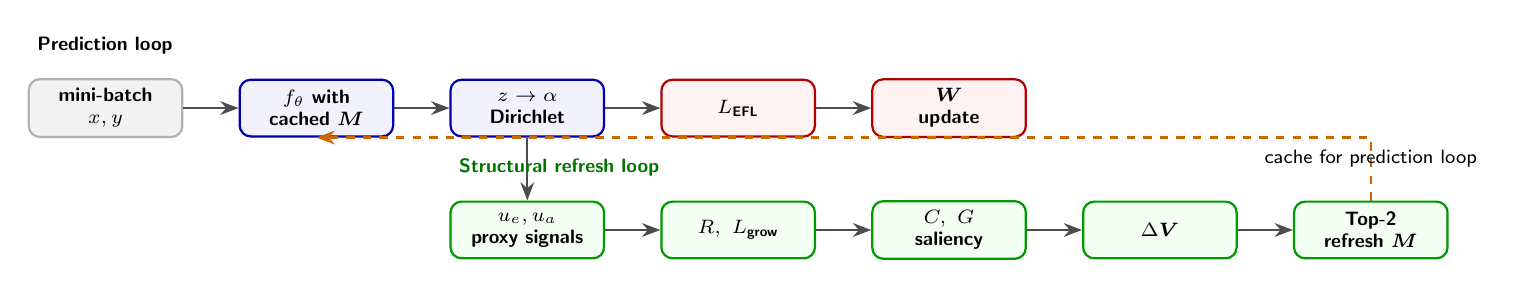
\begin{tikzpicture}[
    node distance=0.8cm and 0.7cm,
    box/.style={
        draw=blue!70!black,
        fill=blue!5,
        rounded corners,
        align=center,
        minimum width=1.95cm,
        minimum height=0.72cm,
        font=\scriptsize\sffamily\bfseries,
        thick
    },
    opt/.style={
        draw=red!70!black,
        fill=red!5,
        rounded corners,
        align=center,
        minimum width=1.95cm,
        minimum height=0.72cm,
        font=\scriptsize\sffamily\bfseries,
        thick
    },
    struct/.style={
        draw=green!60!black,
        fill=green!5,
        rounded corners,
        align=center,
        minimum width=1.95cm,
        minimum height=0.72cm,
        font=\scriptsize\sffamily\bfseries,
        thick
    },
    arrow/.style={
        ->,
        >=Stealth,
        thick,
        draw=black!70
    },
    feedback/.style={
        ->,
        >=Stealth,
        thick,
        dashed,
        draw=orange!80!black
    }
]

% Nodes
\node (x) [box, fill=gray!10, draw=gray!60] {mini-batch\\$x,y$};
\node (f) [box, right=of x] {$f_\theta$ with\\cached $\bm{M}$};
\node (za) [box, right=of f] {$z\to\alpha$\\Dirichlet};
\node (loss) [opt, right=of za] {$L_{\text{EFL}}$};
\node (wup) [opt, right=of loss] {$\bm{W}$\\update};

\node (sig) [struct, below=of za] {$u_e,u_a$\\proxy signals};
\node (risk) [struct, right=of sig] {$R,\ L_{\text{grow}}$};
\node (cg) [struct, right=of risk] {$C,\ G$\\saliency};
\node (dv) [struct, right=of cg] {$\Delta\bm{V}$};
\node (top) [struct, right=of dv] {Top-2\\refresh $\bm{M}$};

% Paths
\draw [arrow] (x) -- (f);
\draw [arrow] (f) -- (za);
\draw [arrow] (za) -- (loss);
\draw [arrow] (loss) -- (wup);
\draw [arrow] (za) -- (sig);
\draw [arrow] (sig) -- (risk);
\draw [arrow] (risk) -- (cg);
\draw [arrow] (cg) -- (dv);
\draw [arrow] (dv) -- (top);
\draw [feedback] (top.north) |- node[above, pos=0.18, font=\scriptsize\sffamily] {cache for prediction loop} (f.south);
\node[font=\scriptsize\sffamily\bfseries, anchor=south west] at ($(x.north west)+(0,0.18)$) {Prediction loop};
\node[font=\scriptsize\sffamily\bfseries, anchor=south west, green!45!black] at ($(sig.north west)+(0,0.18)$) {Structural refresh loop};

\end{tikzpicture}%
}
\caption{Two-loop GUDS-EDL mechanism. The prediction loop updates active weights under a cached mask, while the structural refresh loop uses Dirichlet-derived proxy signals to update latent topology scores and refresh the valid-block 2:4 mask.}
\label{fig:overview}
\end{figure}

\subsection{2:4 Mask-Constrained Sparse Topology}
Following the backbone-agnostic formulation of Evidential Deep Learning~\cite{sensoy2018evidential}, we apply GUDS-EDL to a general feature extractor $f_\theta(\cdot)$ by wrapping the convolutional kernels and linear projection matrices that dominate the parameter count. Prediction weights $\bm{W}^{(l)}$ are optimized by the ordinary training objective, while continuous latent scores $\bm{V}^{(l)}$ determine the binary masks $\bm{M}^{(l)}$. For each wrapped layer, the effective weights are
\begin{equation}\label{eq:wrapped_weights}
    \bm{W}_{\text{eff}}^{(l)}=\bm{W}^{(l)}\odot\bm{M}^{(l)} .
\end{equation}
We enforce NVIDIA 2:4 structured sparsity on eligible complete 4-blocks: in every contiguous valid block of four entries along the flattened inner dimension, exactly two entries remain active. For 2D convolutional layers, $\bm{W}^{(l)} \in \R^{C_{\text{out}}\times C_{\text{in}}\times K_h\times K_w}$ is reshaped to $\bm{W}_{\text{flat}}^{(l)}\in\R^{C_{\text{out}}\times (C_{\text{in}}K_hK_w)}$; linear, MLP, and projection layers already have this row-wise form. If a tensor or trailing segment cannot be decomposed into complete valid 4-blocks, those coordinates are excluded from 2:4 sparsity accounting and kept dense in the implementation. Auxiliary padding, when used for bookkeeping, is never trainable and cannot consume active slots.

The feasible mask set is
\begin{equation}\label{eq:c24}
    \mathcal{C}_{2:4}
    =
    \left\{
    \bm{M}\in\{0,1\}^{d_{\text{out}}\times d_{\text{in}}}:
    \sum_{j=0}^{3} M_{i,4k+j}=2,\ \forall i,k
    \right\}.
\end{equation}
Given a latent score tensor $\bm{V}^{(l)}$, the blockwise mask refresh is
\begin{equation}\label{eq:mask}
    \begin{aligned}
    I_{i,k}^{(l)} &= \TopTwo_{j\in\{0,1,2,3\}}
    V_{\text{flat},i,4k+j}^{(l)},\\
    M_{\text{flat},i,4k+j}^{(l)} &=
    \begin{cases}
        1 & \text{if } j\in I_{i,k}^{(l)},\\
        0 & \text{otherwise.}
    \end{cases}
    \end{aligned}
\end{equation}
The mask is then reshaped back to the original tensor dimensions.

\begin{proposition}[2:4 Feasibility Preservation]
\label{prop:24_feasibility}
Assume each eligible wrapped weight tensor is flattened along its inner dimension so that its valid trainable coordinates decompose into disjoint contiguous 4-blocks. The mask generated by Eq.~\ref{eq:mask} satisfies exact 2:4 sparsity in every complete valid block after each mask refresh. Coordinates outside complete valid blocks are excluded from the 2:4 claim and do not affect the reported valid-block fraction.
\end{proposition}

\subsection{Uncertainty-Guided Pruning and Evidence-Seeking Regrowth}
GUDS-EDL implements topology evolution as a rank-normalized first-order saliency update, matching the implemented training rule and ablation protocol in Appendix~C. It should be read as a practical dynamic sparse training rule, not as a proof of globally optimal sparse architecture search. At each structural refresh, an amortized proxy batch computes two differentiable signals through $\bm{W}_{\text{eff}}$: a batch evidential risk-ratio signal for pruning and an evidence-seeking KL signal for regrowth.

For pruning, we define the proxy-batch evidential risk ratio
\begin{equation}\label{eq:batch_risk}
    R_{\mathcal{B}}
    =
    \frac{1}{|\mathcal{B}|}
    \sum_{n\in\mathcal{B}}
    \frac{u_a^{(n)}}{u_e^{(n)}+\epsilon}.
\end{equation}
With the current mask fixed during the proxy pass, the chain rule gives
\begin{equation}\label{eq:r_chain_main}
    \frac{\partial R_{\mathcal{B}}}{\partial w_{\text{eff},ij}}
    =
    \frac{1}{|\mathcal{B}|}\sum_{n\in\mathcal{B}}
    \left[
    \frac{1}{u_e^{(n)}+\epsilon}\frac{\partial u_a^{(n)}}{\partial w_{\text{eff},ij}}
    -\frac{u_a^{(n)}}{(u_e^{(n)}+\epsilon)^2}
    \frac{\partial u_e^{(n)}}{\partial w_{\text{eff},ij}}
    \right].
\end{equation}
Removing an active connection has first-order effect $\Delta R_{\mathcal B}\approx -w_{ij}\partial R_{\mathcal B}/\partial w_{\text{eff},ij}$. Hence positive $w_{ij}\partial R_{\mathcal B}/\partial w_{\text{eff},ij}$ indicates that setting the connection to zero is locally predicted to reduce the batch risk ratio. The implemented pruning score is
\begin{equation}\label{eq:C_ij}
    C_{ij}
    =
    \operatorname{Rank}_{l}\!\left(
    \pospart{w_{ij}
    \frac{\partial R_{\mathcal B}}{\partial w_{\text{eff},ij}}}
    \right),
    \qquad
    \pospart{x}=\max(x,0).
\end{equation}
Here $\operatorname{Rank}_{l}(\cdot)$ maps scores within layer $l$ to $[0,1]$ by empirical percentile rank over the trainable entries of the corresponding tensor. Larger normalized rank means higher within-layer saliency; the transform preserves ordering but intentionally discards absolute scale and is not an optimality guarantee. Ties are resolved by deterministic tensor ordering in the implementation, and nearly flat score tensors are assigned zero normalized rank before optional exploration. The positive-part operator is not a neural ReLU activation; it gates out connections whose first-order removal would increase the risk ratio.
\begin{equation}\label{eq:rank_def}
    \operatorname{Rank}_{l}(s_{ij})
    =
    \frac{1}{|\Omega_l|-1}
    \sum_{(p,q)\in\Omega_l}
    \mathbb{I}\!\left[\tilde{s}_{pq}<\tilde{s}_{ij}\right],
\end{equation}
where $\Omega_l$ denotes the trainable entries in layer $l$ and $\tilde{s}$ denotes the score after deterministic infinitesimal tie-breaking. If $|\Omega_l|=1$ or the score tensor is numerically flat, the normalized rank is set to zero.

\begin{proposition}[Signed First-Order Pruning Criterion]
\label{prop:signed_pruning}
If $R_{\mathcal B}$ is differentiable with respect to the effective weight and $w_{ij}\frac{\partial R_{\mathcal B}}{\partial w_{\text{eff},ij}}>0$, then removing the connection decreases $R_{\mathcal B}$ to first order. If the product is negative, removal increases $R_{\mathcal B}$ to first order.
\end{proposition}

For regrowth, the implementation uses a KL-to-uniform evidence signal. The full GUDS-EDL run optionally applies class conditioning only as a scalar sample gate; it does not multiply, rescale, or otherwise alter the Dirichlet concentration vector:
\begin{equation}\label{eq:grow_objective}
    L_{\text{grow}}
    =
    \frac{1}{B}\sum_{n=1}^{B}
    g_n^{\text{grow}}\,
    \KL(\Dir(\bm{\alpha}^{(n)})\parallel\Dir(\mathbf{1})),
    \qquad
    g_n^{\text{grow}}
    =
    \begin{cases}
    \bar{\omega}_{y_n}u_e^{(n)}, & \text{class-conditioned regrower},\\
    1, & \text{KL-uniform regrower}.
    \end{cases}
\end{equation}
The regrowth score is the layer-wise rank of the absolute proxy gradient
\begin{equation}\label{eq:G_ij}
    G_{ij}
    =
    \operatorname{Rank}_{l}\!\left(
    \left|
    \frac{\partial L_{\text{grow}}}
    {\partial w_{\text{eff},ij}}
    \right|
    \right).
\end{equation}
This score identifies weights whose effective perturbation has high local influence on the evidence-seeking objective. Dormant links do not receive ordinary task gradients because the mask blocks them. During structural refresh, however, we retain the dense proxy gradient with respect to the effective weight tensor $\bm{W}_{\text{eff}}$ before multiplying it back into the masked parameter gradient. Thus inactive entries can receive structural saliency estimates even though their ordinary training gradients with respect to $\bm{W}$ are zero. When the regrowth signal is nearly flat, a small vacuity-scaled exploration term is used only for tie-breaking. The score does not guarantee that activating a link will improve validation performance; its contribution is evaluated empirically through the no-regrower and KL-uniform-regrower ablations.

\begin{proposition}[Local Regrowth Saliency]
\label{prop:regrowth_saliency}
Let $Q(\bm{W}_{\text{eff}})=L_{\text{grow}}$ be differentiable. Among scalar perturbations $|\delta_{ij}|\le\eta$, the largest first-order change in $Q$ is proportional to $\left|\partial Q/\partial w_{\text{eff},ij}\right|$. Thus Eq.~\ref{eq:G_ij} is a local saliency criterion for candidate structural exploration.
\end{proposition}

The two rank-normalized scores are combined in the latent score update
\begin{equation}\label{eq:score_update}
\begin{aligned}
    \Delta V_{ij}^{(t)}
    &=
    M_{ij}^{(t)}
    \left(G_{ij}^{(t)}-C_{ij}^{(t)}\right)
    +
    \left(1-M_{ij}^{(t)}\right)
    \rho G_{ij}^{(t)}
    + \zeta_{ij}^{(t)},\\
    \mu_{ij}^{(t)} &= \beta_m\mu_{ij}^{(t-1)}+(1-\beta_m)\Delta V_{ij}^{(t)},\\
    X_{ij}^{(t)} &= V_{ij}^{(t-1)}+\eta_{\text{struct}}\mu_{ij}^{(t)},\\
    V_{ij}^{(t)} &=
    \operatorname{clamp}\!\left(
    X_{ij}^{(t)}-\operatorname{mean}(\bm{X}^{(t)}),
    -V_{\max},V_{\max}
    \right).
\end{aligned}
\end{equation}
where $\zeta_{ij}^{(t)}=(1-M_{ij}^{(t)})\xi_{ij}^{(t)}$ is an optional implementation-level perturbation. The pruning term $C_{ij}$ therefore acts only on active links, while dormant links are moved by attenuated regrowth. The coefficient $\rho\in[0,1]$ attenuates dormant-link growth in the implementation. The exploration term $\xi_{ij}^{(t)}$ is not part of the first-order saliency criterion; it is used only as a tie-breaking/anti-crystallization heuristic when rank-normalized regrowth scores are nearly flat. The core GUDS-EDL update is determined by $G$, $C$, the active/dormant mask split, and valid-block Top-2 projection. Since $\bm{V}$ is clamped after every structural update, this perturbation cannot make the structural state unbounded. We report or ablate it separately and do not rely on it for the theoretical validity claims.

\begin{proposition}[Bounded Morphological State]
\label{prop:bounded_scores}
For every structural update using Eq.~\ref{eq:score_update}, all latent scores satisfy $V_{ij}^{(t)}\in[-V_{\max},V_{\max}]$. Therefore, the structural state remains bounded, and every subsequent mask refresh remains feasible under Proposition~\ref{prop:24_feasibility}.
\end{proposition}

\subsection{Gradient Isolation, Caching, and Stability Diagnostics}
Ordinary training uses a fixed cached mask for the mini-batch. Therefore prediction gradients and weight decay only update active links:
\begin{proposition}[Masked-Gradient Isolation]
\label{prop:masked_gradient}
Let $L$ be any differentiable mini-batch training loss evaluated through $\bm{W}_{\text{eff}}=\bm{W}\odot\bm{M}$ with a fixed binary mask $\bm{M}$. Then
\begin{equation}\label{eq:masked_gradient}
    \nabla_{\bm{W}} L
    =
    \nabla_{\bm{W}_{\text{eff}}} L \odot \bm{M}.
\end{equation}
Consequently, inactive entries with $M_{ij}=0$ receive zero ordinary training gradient with respect to $\bm{W}$. The amortized structural proxy gradients above are retained with respect to $\bm{W}_{\text{eff}}$ before applying the masked parameter-gradient identity, and therefore provide a separate saliency route for future regrowth.
\end{proposition}

To avoid sorting and Top-2 operations at every mini-batch, the mask is registered as a non-persistent cache and held fixed between structural refreshes. If an entire layer has near-identical structural scores, GUDS-EDL may add small layer-normalized exploration noise before Eq.~\ref{eq:mask}; this is an implementation device for tie-breaking and anti-crystallization, not a separate optimization objective. Topology variation is monitored by
\begin{equation}\label{eq:flip_rate}
    \operatorname{FlipRate}^{(t)}
    =
    \frac{\|\bm{M}^{(t)}-\bm{M}^{(t-1)}\|_0}
    {\|\bm{M}^{(t-1)}\|_0}.
\end{equation}
A decreasing FlipRate curve is treated as empirical stability evidence, not as a proof of global topology convergence.

\paragraph{Summary of Algorithmic Validity Properties.}
The main theoretical role of this section is deliberately limited. We establish valid Dirichlet-derived signals (Proposition~\ref{prop:evidential_validity}), exact 2:4 feasibility (Proposition~\ref{prop:24_feasibility}), first-order motivation for the signed pruning score (Proposition~\ref{prop:signed_pruning}), local saliency motivation for regrowth (Proposition~\ref{prop:regrowth_saliency}), bounded latent scores (Proposition~\ref{prop:bounded_scores}), and isolation of ordinary training gradients from dormant links (Proposition~\ref{prop:masked_gradient}). These properties make the implemented algorithm well-defined; they do not imply global convergence, optimal sparse architecture discovery, calibrated Bayesian uncertainty, or hardware speedup without sparse Tensor Core-compatible kernels.

\begin{remark}[Role of Residual Connections]
When applied to architectures with residual skip connections, the identity mapping pathways act as safe bypass routes. By preserving identity mapping pathways, they protect spatial information flow from abrupt topological disruption when the network applies valid-block 2:4 structured sparsity.
\end{remark}

\section{Optimization Framework}\label{sec:optimization}

To address extreme class imbalance, we adapt Evidential Focal Loss (EFL) from Zhou et al.~\cite{zhou2023domain}. We acknowledge that the core architecture of combining evidential Dirichlet distributions with focal modulation is their direct contribution. Our implementation uses square-root class-frequency dampening, stop-gradient focal modulation, KL annealing, and a capped asymmetric KL multiplier.

Under extreme long-tail distributions, standard symmetric KL regularization can penalize minority samples disproportionately, encouraging conservative majority-biased predictions. The implemented training objective is
\begin{equation}\label{eq:efl}
\begin{aligned}
    L_{\text{EFL}}(\bm{e}, \bm{y}, t) ={}& \frac{1}{N} \sum_{n=1}^N
    \mathcal{F}_n(t)
    \left[
    \bar{\omega}_{y_n}L_{\text{CE}}^{(n)}
    + \lambda_{\text{KL}}\mu(t)
    \Lambda_{\text{asym}}^{(n)}
    L_{\text{KL}}^{(n)}
    \right].
\end{aligned}
\end{equation}
The dampened class weights are normalized so that the majority class has weight one and then capped:
\begin{equation}\label{eq:sample_weight}
    \omega_c=\sqrt{\frac{N_{\text{majority}}}{N_c}},
    \qquad
    \bar{\omega}_c=\min(\omega_c,\omega_{\max}),
    \qquad
    \omega_{\text{majority}}=1,
    \qquad
    \omega_{\max}=10.0 .
\end{equation}
The square-root form damps inverse-frequency scaling compared with direct inverse prevalence weighting, while the cap makes the imbalance modulation bounded by design. The expected cross-entropy under the Dirichlet predictive distribution is:
\begin{equation}\label{eq:dirichlet_ce}
    L_{\text{CE}}^{(n)}
    = \sum_{c=1}^K y_c^{(n)}
    \left[\psi(S^{(n)})-\psi(\alpha_c^{(n)})\right].
\end{equation}
The focal term is applied with stop-gradient confidence so that focal weighting changes sample emphasis without directly distorting the Dirichlet evidence:
\begin{equation}\label{eq:focal_schedule}
\begin{aligned}
    \mathcal{F}_n(t)
    &= \left(1-\operatorname{sg}\!\left[\hat{p}_{y_n}^{(n)}\right]\right)^{\gamma(t)},\\
    \gamma(t)
    &= \gamma_{\max}\frac{1}{2}\left(1-\cos\left(\pi
    \frac{\max(0,t-T_w)}{T-T_w}\right)\right),
    \qquad \gamma_{\max}=1.2 .
\end{aligned}
\end{equation}
For KL regularization, we remove the true-class evidence from the penalty by defining
$\tilde{\alpha}_c^{(n)}=y_c^{(n)}+(1-y_c^{(n)})\alpha_c^{(n)}$. The adjusted KL term is:
\begin{equation}\label{eq:kl_loss_main}
    L_{\text{KL}}^{(n)}
    =
    \KL\!\left(\Dir(\tilde{\bm{\alpha}}^{(n)})\parallel\Dir(\mathbf{1})\right).
\end{equation}
The annealing coefficient is $\mu(t)=\min(1.0,t/t_{\text{anneal}})$ with $t_{\text{anneal}}=10$. In the reported asymmetric configuration, the additional KL multiplier is capped:
\begin{equation}\label{eq:asym_multiplier}
    \Lambda_{\text{asym}}^{(n)}
    =
    \min(\bar{\omega}_{y_n},\Lambda_{\max}),
    \qquad \Lambda_{\max}=10.0 .
\end{equation}
When the symmetric-KL ablation is used, $\Lambda_{\text{asym}}^{(n)}=1$. Importantly, $\bar{\omega}_{y_n}$ weights the supervised CE term, while $\Lambda_{\text{asym}}^{(n)}$ is the only additional class-dependent multiplier on the KL term; this avoids double-counting the class-frequency weight inside the KL penalty. We do not claim this objective is the unique optimal imbalance correction; its role is evaluated through the symmetric-KL and no-EFL ablations.
The overall training objective is simply
\begin{equation}\label{eq:total_loss}
    L_{\text{total}}=L_{\text{EFL}}(\bm{e},\bm{y},t).
\end{equation}

\begin{proposition}[Controlled Imbalance Modulation]
\label{prop:controlled_modulation}
For each sample $n$, the stop-gradient focal factor $\mathcal{F}_n(t)$ makes the EFL gradient a non-negative sample reweighting of the Dirichlet CE/KL gradients with respect to the evidence parameters, rather than introducing an additional derivative path through $\hat{p}_{y_n}^{(n)}$. The supervised class weight is bounded by $\bar{\omega}_{y_n}\le\omega_{\max}$, and the additional asymmetric KL multiplier is explicitly capped by $\Lambda_{\max}$.
\end{proposition}

\paragraph{Training Warmup.}
We use a short learning-rate and loss-scale warmup for numerical stability. Its schedule is an implementation detail and is given with the full training algorithm in Appendix~B.

\subsection{Post-hoc Calibration and Decision Thresholding}
Post-hoc calibration is applied to logits before the Softplus evidence map. Because this changes both predictive probabilities and Dirichlet strength, we treat it as evidential post-hoc calibration rather than ordinary softmax temperature scaling. The implementation supports temperature-only and bias-temperature modes, with prior-shift correction fitted on the calibration partition; the full formula is given in Appendix~B.

Operating thresholds are selected separately by sweeping validation probabilities $\hat p_c=\alpha_c/S$. Threshold selection changes the decision rule used for Sensitivity/Specificity trade-offs but does not recalibrate the underlying evidence values.

\paragraph{Scope of Claims.}
The theoretical statements above establish that the proposed structural update is well-defined, mask-feasible, and motivated by local first-order saliency under a proper Dirichlet evidence state. They do not prove convergence, optimal topology discovery, Bayesian epistemic correctness, or realized sparse-kernel acceleration. Empirical claims are limited to the reported ISIC 2024 case study; ablations and broader validation protocols are treated as supporting evidence only when explicitly reported.

\section{Experimental Setup}\label{sec:experiment}

\subsection{Evaluation Benchmark}
The main paper reports a high-stakes ISIC 2024 case study. CIFAR-100-LT, additional backbones, and hardware profiling are specified as validation protocols in Appendix~D and are not used to support domain-general claims in the main text.

\paragraph{ISIC 2024 Case Study.} We instantiate GUDS-EDL on the ISIC 2024 Challenge dataset~\cite{isic2024} (3D-TBP images with 0.15\% minority prevalence). To prevent data leakage, we use a stratified 70/5/5/20 train/validation/calibration/test split grouped by patient\_id. The validation partition is used for decision threshold sweeps, the calibration partition for temperature and bias calibration, and the 20\% test partition for final local hold-out evaluation. All images use ImageNet-1K normalization.

\subsection{Baselines and Backbones}
\paragraph{Baselines.} The reported ISIC tables compare evidential baselines for which the same split, calibration protocol, and threshold sweep are available: Fisher EDL, Flexible EDL, R-EDL, and GUDS-EDL. The implemented extended suite additionally includes long-tailed and sparse baselines, but those results are treated as appendix/supplementary validation until fully reported. We therefore do not make SOTA-level claims beyond the evidential comparison.

\paragraph{Backbone Instantiation and Wrapping.}
The reported case study uses a ResNet-18 instantiation. Inside each residual block, the $3 \times 3$ convolutional layers are replaced with sparse convolutional wrappers that apply masks generated by latent scores; the first input convolution is kept dense. The structural proxy pass computes the risk-ratio gradient for the pruner and the KL/evidence gradient for the regrower. Additional grouping diagnostics are documented in Appendix~B and are not separate claimed contributions.

\paragraph{Implementation Details.} Models are trained using 16-bit mixed precision (AMP)~\cite{micikevicius2018mixed}, while evidential losses are evaluated in FP32. We apply square-root balanced sampling on majority classes (subsampled at 1:20 in training) and employ validation-based decision threshold sweeps to select operating points. We compute Expected Calibration Error (ECE) using standard equal-width binning with $M=15$ bins.

\section{Results and Real-World Benchmark Analysis}\label{sec:results}

\subsection{High-Stakes Case Study: ISIC 2024}\label{subsec:isic_case_study}
We report only the latest repeated-seed ISIC results (seeds 42--44). Under this protocol, the default threshold $\tau=0.50$ yields zero minority recall for all four evidential models in every seed, so we focus on the validation-selected balanced operating point together with threshold-independent ranking and calibration metrics.

\begin{table*}[!t]
\centering
\caption{ISIC 2024 repeated-seed results. Values are mean $\pm$ standard deviation over seeds 42--44. Lower AURC and ECE are better.}
\label{tab:isic_repeated_seed_results}
\renewcommand{\arraystretch}{1.10}
\setlength{\tabcolsep}{3.0pt}
\begin{adjustbox}{max width=\textwidth}
\begin{tabular}{l C C C C C C C C}
\toprule
\textbf{Model} & \textbf{Bal. Acc.} $\uparrow$ & \textbf{Sens.} $\uparrow$ & \textbf{Spec.} $\uparrow$ & \textbf{pAUC$_{0.80}$} $\uparrow$ & \textbf{Macro-AUROC} $\uparrow$ & \textbf{PR-AUC} $\uparrow$ & \textbf{AURC} $\downarrow$ & \textbf{ECE} $\downarrow$ \\
\midrule
Fisher EDL   & $0.7359 {\scriptstyle \pm 0.0272}$ & $0.5672 {\scriptstyle \pm 0.0403}$ & $0.9045 {\scriptstyle \pm 0.0813}$ & $0.0428 {\scriptstyle \pm 0.0263}$ & $0.7684 {\scriptstyle \pm 0.0624}$ & $\mathbf{0.0313} {\scriptstyle \pm 0.0035}$ & $0.0006 {\scriptstyle \pm 0.0002}$ & $\mathbf{0.0501} {\scriptstyle \pm 0.0013}$ \\
Flexible EDL & $\mathbf{0.7897} {\scriptstyle \pm 0.0660}$ & $\mathbf{0.6496} {\scriptstyle \pm 0.1655}$ & $0.9299 {\scriptstyle \pm 0.0406}$ & $\mathbf{0.0650} {\scriptstyle \pm 0.0247}$ & $\mathbf{0.8308} {\scriptstyle \pm 0.0428}$ & $0.0243 {\scriptstyle \pm 0.0043}$ & $0.0005 {\scriptstyle \pm 0.0002}$ & $0.0508 {\scriptstyle \pm 0.0021}$ \\
R-EDL        & $0.7605 {\scriptstyle \pm 0.0381}$ & $0.5703 {\scriptstyle \pm 0.0721}$ & $\mathbf{0.9508} {\scriptstyle \pm 0.0103}$ & $0.0396 {\scriptstyle \pm 0.0140}$ & $0.7702 {\scriptstyle \pm 0.0378}$ & $0.0291 {\scriptstyle \pm 0.0044}$ & $0.0006 {\scriptstyle \pm 0.0002}$ & $0.0510 {\scriptstyle \pm 0.0021}$ \\
\midrule
\textbf{GUDS-EDL (Ours)} & $0.7879 {\scriptstyle \pm 0.0118}$ & $0.6309 {\scriptstyle \pm 0.0407}$ & $0.9449 {\scriptstyle \pm 0.0187}$ & $0.0592 {\scriptstyle \pm 0.0064}$ & $0.8188 {\scriptstyle \pm 0.0180}$ & $\mathbf{0.0313} {\scriptstyle \pm 0.0038}$ & $\mathbf{0.0004} {\scriptstyle \pm 0.0002}$ & $0.0553 {\scriptstyle \pm 0.0019}$ \\
\bottomrule
\end{tabular}
\end{adjustbox}
\end{table*}

Table~\ref{tab:isic_repeated_seed_results} shows that the strongest dense baseline is Flexible EDL, which achieves the highest mean Balanced Accuracy, pAUC$_{0.80}$, and Macro-AUROC. GUDS-EDL is slightly behind on those three ranking metrics, but remains competitive while preserving high specificity and attaining the best mean AURC. GUDS-EDL also matches the best mean PR-AUC and exhibits much smaller seed-to-seed variance than Flexible EDL on Balanced Accuracy, pAUC$_{0.80}$, and Macro-AUROC. This is the main positive result of the new evaluation: uncertainty-guided sparse topology adaptation remains competitive under severe imbalance without becoming numerically unstable.

The structural diagnostics are favorable. In all three GUDS-EDL runs, the log reports exact $50.0\%$ sparsity in the wrapped layers, full valid-block feasibility ($2789632/2789632$ valid 2:4 blocks), and no detected representational collapse. These diagnostics matter because they show that the ranking behavior in Table~\ref{tab:isic_repeated_seed_results} is not obtained by an unstable sparse morphology.

The main weakness is calibration and operating-point fragility. GUDS-EDL has the worst mean ECE in Table~\ref{tab:isic_repeated_seed_results}, and its post-hoc temperature repeatedly saturates at the lower bound $T_{\mathrm{cal}}=0.10$ in all three seeds. Together with the universal failure of the default threshold, this indicates that the current evidential scale is not directly deployment ready. In addition, the quality-gated mode discards a larger fraction of cases than the dense baselines while still sacrificing minority sensitivity, so the present abstention rule should be interpreted as preliminary.

Overall, the updated evidence supports a narrower claim than the previous draft. GUDS-EDL is not the best model on every ISIC metric, but it is a competitive sparse evidential model with strong risk-coverage ordering, high specificity, stable repeated-seed behavior, and clean 2:4 structural diagnostics. Its remaining weaknesses are calibration quality and threshold sensitivity under extreme prevalence.

\section{Limitations and Broader Impact}\label{sec:limitations}
Key limitations of the current framework include: (1) empirical validation is currently centered on the ISIC 2024 case study; (2) GUDS-EDL enforces a fixed Top-2-of-4 pattern over eligible complete blocks after warmup, whereas early stages might benefit from an annealed sparsity schedule; (3) while valid-block 2:4 structured sparsity reduces active density in wrapped layers, achieving real hardware acceleration requires specialized 2:4 sparse Tensor Core kernels; (4) minority-class probability calibration remains challenging under extreme prevalence shifts even when rare-event ranking improves; (5) the repeated-seed diagnostic run shows that the method can become strongly threshold dependent, with post-hoc temperature calibration repeatedly saturating at its lower bound and fail-safe thresholds occasionally degenerating into an almost-always-positive classifier; (6) the current uncertainty-gated abstention mode removes only a small fraction of cases while still sacrificing substantial minority recall; and (7) the current implementation includes a small exploration perturbation for anti-crystallization under near-flat structural scores, so future versions should replace it with deterministic tie-breaking or report dedicated sensitivity analysis.

Rare-event learning systems deployed in high-stakes domains carry significant societal responsibility. A primary risk is the extreme cost of false negatives; thus, such models must act as decision-support tools that integrate selective classification to route ambiguous cases to human experts. Algorithmic bias is also a concern: dermatological datasets are often heavily skewed toward lighter Fitzpatrick skin types, and performance may not generalize equally to patients with darker skin tones.

\section{Conclusion}\label{sec:conclusion}
We introduced GUDS-EDL, an uncertainty-guided dynamic sparse evidential learning framework for extreme imbalanced classification. In the updated three-seed ISIC evaluation, GUDS-EDL is competitive with the strongest dense evidential baselines while maintaining exact valid-block 2:4 sparsity, the best mean AURC, and stable structural diagnostics without detected collapse. The same evaluation also shows that calibration quality and threshold sensitivity remain the main open problems. Broader validation on controlled long-tailed recognition, industrial anomaly detection, additional backbones, ablations, and hardware-accelerated sparse kernels remains necessary before claiming domain-general deployment readiness.

\begin{thebibliography}{10}\itemsep=-1pt

\bibitem{guo2017calibration}
C.~Guo, G.~Pleiss, Y.~Sun, and K.~Q. Weinberger.
\newblock On calibration of modern neural networks.
\newblock In {\em International Conference on Machine Learning (ICML)}, 2017.

\bibitem{sensoy2018evidential}
M.~Sensoy, L.~Kaplan, and M.~Kandemir.
\newblock Evidential deep learning to quantify classification uncertainty.
\newblock In {\em Advances in Neural Information Processing Systems (NeurIPS)}, 2018.

\bibitem{malinin2018predictive}
A.~Malinin and M.~Gales.
\newblock Predictive uncertainty estimation via prior networks.
\newblock In {\em Advances in Neural Information Processing Systems (NeurIPS)}, 2018.

\bibitem{evci2020rigging}
U.~Evci, T.~Gale, J.~Menick, P.~S. Castro, and E.~Elsen.
\newblock Rigging the lottery: Making all tickets winners.
\newblock In {\em International Conference on Machine Learning (ICML)}, 2020.

\bibitem{cui2019class}
Y.~Cui, M.~Jia, T.-Y. Lin, Y.~Song, and S.~Belongie.
\newblock Class-balanced loss based on effective number of samples.
\newblock In {\em IEEE/CVF Conference on Computer Vision and Pattern Recognition (CVPR)}, 2019.

\bibitem{cao2019learning}
K.~Cao, C.~Wei, A.~Gaidon, N.~Arechiga, and T.~Ma.
\newblock Learning imbalanced datasets with label-distribution-aware margin loss.
\newblock In {\em Advances in Neural Information Processing Systems (NeurIPS)}, 2019.

\bibitem{menon2021long}
A.~K. Menon, S.~Jayasumana, A.~S. Rawat, H.~Jain, A.~Veit, and S.~Kumar.
\newblock Long-tail learning via logit adjustment.
\newblock In {\em International Conference on Learning Representations (ICLR)}, 2021.

\bibitem{ren2020balanced}
J.~Ren, C.~Yu, S.~Sheng, X.~Ma, H.~Zhao, S.~Yi, and H.~Li.
\newblock Balanced meta-softmax for long-tailed visual recognition.
\newblock In {\em Advances in Neural Information Processing Systems (NeurIPS)}, 2020.

\bibitem{kang2019decoupling}
B.~Kang, S.~Xie, M.~Rohrbach, Z.~Yan, A.~Gordo, J.~Feng, and Y.~Kalantidis.
\newblock Decoupling representation and classifier for long-tailed recognition.
\newblock In {\em International Conference on Learning Representations (ICLR)}, 2020.

\bibitem{zhong2021improving}
Z.~Zhong, J.~Cui, S.~Liu, and J.~Jia.
\newblock Improving calibration for long-tailed recognition.
\newblock In {\em IEEE/CVF Conference on Computer Vision and Pattern Recognition (CVPR)}, 2021.

\bibitem{zhou2020bbn}
B.~Zhou, Q.~Cui, X.-S. Wei, and Z.-M. Chen.
\newblock BBN: Bilateral-branch network with cumulative learning for long-tailed visual recognition.
\newblock In {\em IEEE/CVF Conference on Computer Vision and Pattern Recognition (CVPR)}, 2020.

\bibitem{cui2021parametric}
J.~Cui, Z.~Zhong, S.~Liu, B.~Yu, and J.~Jia.
\newblock Parametric contrastive learning.
\newblock In {\em IEEE/CVF International Conference on Computer Vision (ICCV)}, 2021.

\bibitem{deng2023fisher}
D.~Deng, G.~Chen, Y.~Yu, F.~Liu, and P.-A. Heng.
\newblock Uncertainty estimation by Fisher information-based evidential deep learning.
\newblock In {\em International Conference on Machine Learning (ICML)}, PMLR, 2023.

\bibitem{chen2023redl}
M.~Chen, J.~Gao, and C.~Xu.
\newblock R-EDL: Relaxing nonessential settings of evidential deep learning.
\newblock In {\em International Conference on Learning Representations (ICLR)}, 2024.

\bibitem{chen2024reedl}
M.~Chen, J.~Gao, and C.~Xu.
\newblock Revisiting essential and nonessential settings of evidential deep learning.
\newblock {\em arXiv preprint arXiv:2410.00393}, 2024.

\bibitem{yoon2025flexible}
T.~Yoon and H.~Kim.
\newblock Uncertainty estimation by flexible evidential deep learning.
\newblock {\em arXiv preprint arXiv:2510.18322}, 2025.

\bibitem{yu2024anedl}
Y.~Yu, D.~Deng, F.~Liu, Y.~Jin, Q.~Dou, G.~Chen, and P.-A. Heng.
\newblock ANEDL: Adaptive negative evidential deep learning for open-set semi-supervised learning.
\newblock In {\em AAAI Conference on Artificial Intelligence}, 2024.

\bibitem{wu2024evidence}
Y.~Wu, B.~Shi, B.~Dong, Q.~Zheng, and H.~Wei.
\newblock The evidence contraction issue in deep evidential regression: Discussion and solution.
\newblock In {\em AAAI Conference on Artificial Intelligence}, 2024.

\bibitem{shen2024mirage}
M.~Shen, J.~J. Ryu, S.~Ghosh, Y.~Bu, P.~Sattigeri, S.~Das, and G.~W. Wornell.
\newblock Are uncertainty quantification capabilities of evidential deep learning a mirage?
\newblock In {\em Advances in Neural Information Processing Systems (NeurIPS)}, 2024.

\bibitem{geifman2017selective}
Y.~Geifman and R.~El-Yaniv.
\newblock Selective classification for deep neural networks.
\newblock In {\em Advances in Neural Information Processing Systems (NeurIPS)}, 2017.

\bibitem{geifman2019selectivenet}
Y.~Geifman and R.~El-Yaniv.
\newblock SelectiveNet: A deep neural network with an integrated reject option.
\newblock In {\em International Conference on Machine Learning (ICML)}, 2019.

\bibitem{ding2020revisiting}
Y.~Ding, J.~Liu, J.~Xiong, and Y.~Shi.
\newblock Revisiting the evaluation of uncertainty estimation and its application to explore model complexity-uncertainty trade-off.
\newblock In {\em IEEE/CVF Conference on Computer Vision and Pattern Recognition Workshops (CVPRW)}, 2020.

\bibitem{traub2024overcoming}
J.~Traub, T.~J. Bungert, C.~T. L{\"u}th, M.~Baumgartner, K.~H. Maier-Hein, L.~Maier-Hein, and P.~F. Jaeger.
\newblock Overcoming common flaws in the evaluation of selective classification systems.
\newblock In {\em Advances in Neural Information Processing Systems (NeurIPS)}, 2024.

\bibitem{dettmers2019sparse}
T.~Dettmers and L.~Zettlemoyer.
\newblock Sparse networks from scratch: Faster training without losing performance.
\newblock In {\em ICLR Workshop}, 2019.

\bibitem{lee2019snip}
N.~Lee, T.~Ajanthan, and P.~H.~S. Torr.
\newblock SNIP: Single-shot network pruning based on connection sensitivity.
\newblock In {\em International Conference on Learning Representations (ICLR)}, 2019.

\bibitem{li2025pffdst}
L.~Li, H.~Yang, J.~Guo, H.~Yu, M.~Qin, and T.~Zhang.
\newblock An efficient and accurate dynamic sparse training framework based on parameter-freezing.
\newblock In {\em AAAI Conference on Artificial Intelligence}, 2025.

\bibitem{lasby2023srigl}
M.~Lasby, A.~Golubeva, U.~Evci, M.~Nica, and Y.~Ioannou.
\newblock Dynamic sparse training with structured sparsity.
\newblock In {\em International Conference on Learning Representations (ICLR)}, 2024.

\bibitem{mishra2021accelerating}
Asit Mishra, Jorge Albericio Latorre, Jeff Pool, Darko Stosic, Dusan Stosic, Ganesh Venkatesh, Chong Yu, and Paulius Micikevicius.
\newblock Accelerating sparse deep neural networks.
\newblock {\em arXiv preprint arXiv:2104.08378}, 2021.

\bibitem{mocanu2018scalable}
D.~C. Mocanu, E.~Mocanu, P.~Stone, P.~H. Nguyen, M.~Gibescu, and A.~Liotta.
\newblock Scalable training of artificial neural networks with adaptive sparse connectivity inspired by network science.
\newblock {\em Nature Communications}, 9(1):2383, 2018.

\bibitem{han2016deep}
S.~Han, H.~Mao, and W.~J. Dally.
\newblock Deep compression: Compressing deep neural networks with pruning, trained quantization and Huffman coding.
\newblock In {\em International Conference on Learning Representations (ICLR)}, 2016.

\bibitem{frankle2019lottery}
J.~Frankle and M.~Carbin.
\newblock The lottery ticket hypothesis: Finding sparse, trainable neural networks.
\newblock In {\em International Conference on Learning Representations (ICLR)}, 2019.

\bibitem{liu2019large}
Z.~Liu, Z.~Miao, X.~Zhan, J.~Wang, B.~Gong, and S.~X. Yu.
\newblock Large-scale long-tailed recognition in an open world.
\newblock In {\em IEEE/CVF Conference on Computer Vision and Pattern Recognition (CVPR)}, 2019.

\bibitem{roth2022total}
K.~Roth, L.~Pemula, J.~Zepeda, B.~Sch{\"o}lkopf, T.~Brox, and P.~Gehler.
\newblock Towards total recall in industrial anomaly detection.
\newblock In {\em IEEE/CVF Conference on Computer Vision and Pattern Recognition (CVPR)}, 2022.

\bibitem{isic2024}
International Skin Imaging Collaboration (ISIC).
\newblock ISIC 2024 -- Skin Cancer Detection with 3D-TBP.
\newblock {\em Kaggle Competition}, 2024.

\bibitem{jaeger2023call}
P.~F. Jaeger, C.~T. L{\"u}th, L.~Klein, and T.~J. Bungert.
\newblock A call to reflect on evaluation practices for failure detection in image classification.
\newblock In {\em International Conference on Learning Representations (ICLR)}, 2023.

\bibitem{zhou2023domain}
M.~Zhou, A.~Jamzad, J.~Izard, A.~Menard, R.~Siemens, and P.~Mousavi.
\newblock Domain transfer through image-to-image translation for uncertainty-aware prostate cancer classification.
\newblock {\em arXiv preprint arXiv:2307.00479}, 2023.

\bibitem{micikevicius2018mixed}
P.~Micikevicius, S.~Narang, J.~Alben, G.~Diamos, E.~Elsen, D.~Garcia, B.~Ginsburg, M.~Houston, O.~Kuchaiev, G.~Venkatesh, and H.~Wu.
\newblock Mixed precision training.
\newblock In {\em International Conference on Learning Representations (ICLR)}, 2018.

\bibitem{loshchilov2019decoupled}
I.~Loshchilov and F.~Hutter.
\newblock Decoupled weight decay regularization.
\newblock In {\em International Conference on Learning Representations (ICLR)}, 2019.

\bibitem{kingma2015adam}
D.~P. Kingma and J.~Ba.
\newblock Adam: A method for stochastic optimization.
\newblock In {\em International Conference on Learning Representations (ICLR)}, 2015.

\bibitem{charpentier2020posterior}
B.~Charpentier, D.~Z{\"u}gner, and S.~G{\"u}nnemann.
\newblock Posterior Network: Uncertainty estimation without OOD samples via density-based pseudo-counts.
\newblock In {\em Advances in Neural Information Processing Systems (NeurIPS)}, 2020.

\end{thebibliography}

\appendix

\section{Appendix A: Proofs and Mathematical Derivations}
\label{app:proofs}

\subsection{Compact Dirichlet Identities}
For completeness, the Dirichlet density for $\bm{p}$ on the probability simplex is
\begin{equation}\label{eq:dirichlet_pdf_app}
    \Dir(\bm{p}\mid\bm{\alpha})
    =
    \frac{1}{B(\bm{\alpha})}\prod_{c=1}^{K}p_c^{\alpha_c-1}
    =
    \frac{\Gamma(S)}{\prod_{c=1}^{K}\Gamma(\alpha_c)}
    \prod_{c=1}^{K}p_c^{\alpha_c-1}.
\end{equation}
The implementation uses the following identities from the main text:
\begin{equation}
    \hat{p}_c=\frac{\alpha_c}{S},\qquad
    u_e=\frac{K}{S},\qquad
    u_a=\sum_{c=1}^{K}\frac{\alpha_c}{S}
    \left[\psi(S+1)-\psi(\alpha_c+1)\right].
\end{equation}
Under the Softplus evidence parameterization, $\alpha_c>1$ and therefore $S>K$ for finite logits. Hence $u_e\in(0,1)$, with supremum $1$ approached as all evidence tends to zero. Since $S\ge \alpha_c$ and $\psi(\cdot)$ is monotone on positive inputs, each entropy summand is non-negative, so $u_a\ge0$.

\subsection{Structural Risk-Ratio Chain Rule}
\label{app:r_chain}
The batch structural risk ratio $R_{\mathcal B}$ in Eq.~\ref{eq:batch_risk} is differentiable for $\epsilon>0$ under the Softplus evidence map when the current mask is held fixed during the proxy structural pass. Its weight derivative is the batch average of the per-sample ratio derivatives:
\begin{equation}
    \frac{\partial R_{\mathcal B}}{\partial w_{ij}}
    =
    \frac{1}{|\mathcal B|}\sum_{n\in\mathcal B}
    \left[
    \frac{1}{u_e+\epsilon}\frac{\partial u_a}{\partial w_{ij}}
    -
    \frac{u_a}{(u_e+\epsilon)^2}
    \frac{\partial u_e}{\partial w_{ij}}
    \right]^{(n)} .
\end{equation}
The vacuity derivative expands through the Dirichlet parameters as
\begin{equation}
    \frac{\partial u_e}{\partial w_{ij}}
    =
    \sum_{m=1}^{K}
    \frac{\partial u_e}{\partial \alpha_m}
    \frac{\partial \alpha_m}{\partial z_m}
    \frac{\partial z_m}{\partial w_{ij}},
    \qquad
    \frac{\partial u_e}{\partial \alpha_m}
    =
    -\frac{K}{S^2},
\end{equation}
where $\frac{\partial \alpha_m}{\partial z_m}=1/(1+\exp(-z_m))$ for $\alpha_m=\ln(1+\exp(z_m))+1$. For the entropy proxy, let $\psi_1(\cdot)$ denote the trigamma function and $\delta_{cm}$ the Kronecker delta. Then
\begin{equation}
\begin{aligned}
    \frac{\partial u_a}{\partial \alpha_m}
    ={}&
    \sum_{c=1}^{K}
    \frac{\delta_{cm}S-\alpha_c}{S^2}
    \left[\psi(S+1)-\psi(\alpha_c+1)\right]\\
    &+
    \sum_{c=1}^{K}
    \frac{\alpha_c}{S}
    \left[
    \psi_1(S+1)-\delta_{cm}\psi_1(\alpha_c+1)
    \right],
\end{aligned}
\end{equation}
and therefore
\begin{equation}
    \frac{\partial u_a}{\partial w_{ij}}
    =
    \sum_{m=1}^{K}
    \frac{\partial u_a}{\partial \alpha_m}
    \frac{\partial \alpha_m}{\partial z_m}
    \frac{\partial z_m}{\partial w_{ij}} .
\end{equation}
This expansion provides the batch risk-ratio derivative used by the signed pruning score in Eq.~\ref{eq:C_ij}. It combines local vacuity and expected-entropy derivatives through the ordinary network Jacobian $\partial z_m/\partial w_{ij}$, rather than relying on an unspecified pruning signal.

\subsection{Asymmetric KL Note}
The adjusted false-evidence parameter $\tilde{\alpha}_c^{(n)}=y_c^{(n)}+(1-y_c^{(n)})\alpha_c^{(n)}$ defines the compact KL term in Eq.~\ref{eq:kl_loss_main}. Its expanded form is the standard Dirichlet-to-Dirichlet KL with the true-class concentration removed from the shrinkage penalty:
\begin{equation}\label{eq:kl_loss_expanded}
\begin{aligned}
    L_{\text{KL}}^{(n)}
    ={}& \ln \left(
    \frac{\Gamma\left(\sum_{c=1}^K\tilde{\alpha}_c^{(n)}\right)}
    {\Gamma(K)\prod_{c=1}^K\Gamma(\tilde{\alpha}_c^{(n)})}
    \right)\\
    &+\sum_{c=1}^K(\tilde{\alpha}_c^{(n)}-1)
    \left[
    \psi(\tilde{\alpha}_c^{(n)})
    -\psi\!\left(\sum_{c=1}^K\tilde{\alpha}_c^{(n)}\right)
    \right].
\end{aligned}
\end{equation}

\subsection{Proof of Proposition~\ref{prop:evidential_validity}}
Softplus is strictly positive for finite real-valued logits, hence $\alpha_c=e_c+1>1$ and $S=\sum_c\alpha_c>K$. The expected probabilities obey $\hat{p}_c=\alpha_c/S>0$ and $\sum_c\hat{p}_c=1$, so $\hat{\bm{p}}\in\Delta^K$. Since $S>K$, $u_e=K/S\in(0,1)$ for finite logits, with limiting value $1$ approached when all evidence values $e_c$ tend to zero. Finally, $S\ge\alpha_c$ for every class and $\psi(\cdot)$ is monotone on positive inputs. Therefore $\psi(S+1)-\psi(\alpha_c+1)\ge0$, and each summand in Eq.~\ref{eq:u_a} is non-negative. Hence $u_a\ge0$.

\subsection{Proof of Proposition~\ref{prop:24_feasibility}}
For each eligible row $i$ and complete valid block $k$, Eq.~\ref{eq:mask} selects the two local indices in $I_{i,k}^{(l)}$ and assigns mask value $1$ only to those entries. The remaining two entries receive mask value $0$. Auxiliary padding entries, if used for bookkeeping, have score $-\infty$ and are not trainable; they cannot be selected and cannot consume active slots. Hence every complete valid 4-block contains exactly two active trainable entries. Coordinates outside complete valid blocks are excluded from the exact 2:4 claim and are reported through the valid-block fraction rather than folded into the numerator or denominator of the structured-sparsity guarantee.

\subsection{Proof of Proposition~\ref{prop:masked_gradient}}
For each entry, $W_{\text{eff},ij}=W_{ij}M_{ij}$ while the mask is fixed during the mini-batch. By the chain rule,
\begin{equation}
    \frac{\partial L}{\partial W_{ij}}
    =
    \frac{\partial L}{\partial W_{\text{eff},ij}}
    \frac{\partial W_{\text{eff},ij}}{\partial W_{ij}}
    =
    \frac{\partial L}{\partial W_{\text{eff},ij}}M_{ij}.
\end{equation}
Stacking this entry-wise identity over the tensor gives Eq.~\ref{eq:masked_gradient}. If $M_{ij}=0$, the instantaneous task gradient with respect to $W_{ij}$ is zero, which motivates the separate structural proxy pass used by the pruning/regrowth update.

\subsection{Proof of Proposition~\ref{prop:signed_pruning}}
The first-order Taylor expansion of $R_{\mathcal B}$ after replacing $w_{ij}$ by $0$ is
\begin{equation}
    R_{\mathcal B}(w_{ij}=0)-R_{\mathcal B}(w_{ij})
    =
    -w_{ij}\frac{\partial R_{\mathcal B}}{\partial w_{\text{eff},ij}}
    + o(|w_{ij}|).
\end{equation}
The leading term is negative exactly when $w_{ij}\frac{\partial R_{\mathcal B}}{\partial w_{\text{eff},ij}}>0$. Thus, to first order, removing such a connection decreases the batch evidential risk ratio. Conversely, when the product is negative, the leading term is positive and removal increases the risk ratio. The positive-part operator in Eq.~\ref{eq:C_ij} keeps only the first case as a pruning candidate.

\subsection{Proof of Proposition~\ref{prop:regrowth_saliency}}
Let $Q(\bm{W}_{\text{eff}})=L_{\text{grow}}(\bm{W}_{\text{eff}})$. For a scalar perturbation $\delta_{ij}$ at connection $(i,j)$,
\begin{equation}
    Q(w_{\text{eff},ij}+\delta_{ij})-Q(w_{\text{eff},ij})
    =
    \delta_{ij}\frac{\partial Q}{\partial w_{\text{eff},ij}}
    + o(|\delta_{ij}|).
\end{equation}
Under the constraint $|\delta_{ij}|\le\eta$, the absolute value of the leading term is maximized by choosing $\delta_{ij}=\eta\,\operatorname{sign}(\partial Q/\partial w_{\text{eff},ij})$, yielding $\eta\left|\frac{\partial Q}{\partial w_{\text{eff},ij}}\right|$. Therefore, ranking candidates by Eq.~\ref{eq:G_ij} selects entries with high local first-order ability to alter the evidence-seeking objective.

\subsection{Proof of Proposition~\ref{prop:bounded_scores}}
The final operation in Eq.~\ref{eq:score_update} applies an element-wise clamp to the interval $[-V_{\max},V_{\max}]$. Hence every updated score lies in that interval regardless of the magnitude of the unclamped momentum step. The mask is then recomputed from the bounded score tensor using Eq.~\ref{eq:mask}, so Proposition~\ref{prop:24_feasibility} applies at the next refresh.

\subsection{Proof of Proposition~\ref{prop:controlled_modulation}}
Because $\operatorname{sg}[\hat{p}_{y_n}^{(n)}]$ is treated as constant during backpropagation, $\nabla_{\bm{e}}\mathcal{F}_n(t)=0$. Thus the sample-level gradient is proportional to
\begin{equation}
    \mathcal{F}_n(t)
    \nabla_{\bm{e}}\!\left(
    \bar{\omega}_{y_n}L_{\text{CE}}^{(n)}
    +\lambda_{\text{KL}}\mu(t)\Lambda_{\text{asym}}^{(n)}
    L_{\text{KL}}^{(n)}
    \right).
\end{equation}
Moreover, $\mathcal{F}_n(t)\ge0$, $\mu(t)\in[0,1]$, $\bar{\omega}_{y_n}\le\omega_{\max}$ by Eq.~\ref{eq:sample_weight}, and $\Lambda_{\text{asym}}^{(n)}\le\Lambda_{\max}$ by Eq.~\ref{eq:asym_multiplier}. Hence focal modulation changes sample emphasis without adding an uncontrolled confidence-derivative path, while both the supervised class weight and the additional asymmetric KL multiplier are explicitly capped.

\FloatBarrier
\section{Appendix B: Full GUDS-EDL Algorithm and Implementation}
\paragraph{Learning-rate and loss-scale warmup.}
During the first epoch, the learning rate is linearly warmed from $\eta_{\text{init}}=10^{-6}$ to $\eta_{\text{base}}=4\times10^{-5}$, while an initial loss multiplier decays from $S_{\max}=4.0$ to $1.0$:
\begin{equation}\label{eq:warmup_main}
    \eta_s=\eta_{\text{init}}+(\eta_{\text{base}}-\eta_{\text{init}})
    \frac{s}{S_{\text{warmup}}},
    \qquad
    S_{\text{loss}}(s)=S_{\max}-(S_{\max}-1)
    \frac{s}{S_{\text{warmup}}}.
\end{equation}
The scaled objective $L_{\text{scaled}}=S_{\text{loss}}(s)L_{\text{total}}$ is used during warmup and $L_{\text{total}}$ afterward.

\paragraph{Bias-corrected evidential calibration.}
After training, logits are corrected before the Softplus evidence map by
\begin{equation}
    z^{\mathrm{cal}}_c
    =
    \frac{z^{\mathrm{base}}_c+\Delta^\pi_c}{T_{\mathrm{cal}}}
    + b_{\mathrm{res},c},
    \qquad
    \Delta^\pi_c=\log(\pi_{\mathrm{true},c}+\epsilon)-\log(\pi_{\mathrm{train},c}+\epsilon).
\end{equation}
Temperature-only calibration sets $\bm{b}_{\mathrm{res}}=\bm{0}$; bias-temperature calibration learns both $T_{\mathrm{cal}}$ and $\bm{b}_{\mathrm{res}}$ on the calibration partition.

\begin{algorithm}[H]
\caption{GUDS-EDL Training and Optimization Loop}
\label{alg:guds_edl}
\begin{algorithmic}[1]
\REQUIRE Dataset $\mathcal{D}$, weights $\bm{W}^{(0)}$, latent scores $\bm{V}^{(0)}\leftarrow|\bm{W}^{(0)}|$, structural momentum $\bm{\mu}^{(0)}\leftarrow\bm{0}$, epochs $T$, warmup epochs $T_w$.
\FOR{each epoch $t = 1 \dots T$}
    \IF{$t == T_w$}
        \STATE Optionally freeze learned channel permutations into static index maps for 2:4 block ordering.
    \ENDIF
    \IF{$t \ge T_w$}
        \STATE Sample a proxy batch $(\bm{X}, \bm{y}) \sim \mathcal{D}$ for amortized topology computation.
        \STATE Compute $R_{\mathcal B}$ by Eq.~\ref{eq:batch_risk} and store $\nabla_{\bm{W}_{\text{eff}}}R_{\mathcal B}$ for the pruner.
        \STATE Compute $L_{\text{grow}}$ by Eq.~\ref{eq:grow_objective} and store $\nabla_{\bm{W}_{\text{eff}}}L_{\text{grow}}$ for the regrower.
        \STATE Compute $C_{ij}$ by Eq.~\ref{eq:C_ij} and $G_{ij}$ by Eq.~\ref{eq:G_ij}.
        \STATE Optionally add vacuity-scaled exploration noise when $G_{ij}$ is nearly flat.
        \STATE Update active and dormant latent scores $\bm{V}$ by Eq.~\ref{eq:score_update}.
        \STATE Refresh and cache $\bm{M}^{(l)}$ by 2:4 Top-2 selection in Eq.~\ref{eq:mask}.
    \ELSE
        \STATE Set masks $\bm{M}^{(l)}\leftarrow\mathbf{1}$ for dense warmup.
    \ENDIF
    \FOR{each mini-batch step $s$ in epoch $t$}
        \STATE Sample batch $(\bm{X}, \bm{y}) \sim \mathcal{D}$.
        \STATE Compute $\eta_s$ and $S_{\text{loss}}(s)$ by Eq.~\ref{eq:warmup_main}.
        \STATE Forward pass: compute logits $\bm{z}$ using static masked weights $\bm{W}_{\text{eff}} = \bm{W} \odot \bm{M}$.
        \STATE Compute Dirichlet parameters: $\alpha_c \leftarrow \ln(1 + e^{z_c}) + 1.0$.
        \STATE Compute expected probabilities $\hat{p}_c = \alpha_c/S$ and uncertainties $u_e, u_a$.
        \STATE Compute $L_{\text{scaled}}=S_{\text{loss}}(s)L_{\text{EFL}}$ using Eq.~\ref{eq:efl}.
        \STATE Backward pass and update active weights with AdamW under the fixed cached mask.
    \ENDFOR
\ENDFOR
\end{algorithmic}
\end{algorithm}

\begin{table}[H]
\centering
\caption{Hyperparameter and implementation configuration for the ISIC 2024 case study. $T$ denotes total training epochs, while $T_{\text{cal}}$ denotes the post-hoc calibration temperature.}
\label{tab:config}
\scriptsize
\renewcommand{\arraystretch}{0.9}
\setlength{\tabcolsep}{2.0pt}
\begin{adjustbox}{max width=\columnwidth,max totalheight=0.92\textheight}
\begin{tabular}{@{}p{0.27\columnwidth}p{0.24\columnwidth}p{0.39\columnwidth}@{}}
\toprule
\textbf{Phase / Component} & \textbf{Parameter} & \textbf{Role Description} \\
\midrule
\multicolumn{3}{l}{\emph{Architecture}} \\
Backbone & ResNet-18 (11.7M params) & ImageNet-1K pretrained \\
Number of Classes ($K$) & 2 & Benign / Malignant \\
\midrule
\multicolumn{3}{l}{\emph{Phase 1: Dense Warmup ($t < T_w$)}} \\
Mask & Locked entirely at $\bm{1}$ & Dense network, no pruning \\
Focal exponent $\gamma(t)$ & $0.0$ & Disabled for baseline convergence stability \\
\midrule
\multicolumn{3}{l}{\emph{Phase 2: Dynamic Sparsity ($t \ge T_w$)}} \\
Mask & NVIDIA 2:4 & Top-2-of-4 from latent scores $\bm{V}$ \\
Topology Adaptation & Activated & Update $\bm{V}$ and $\bm{M}$ once per epoch using a proxy batch \\
$\gamma_{\text{focal}}$ & Linear $\to 1.2$ & Focus on hard samples \\
\midrule
\multicolumn{3}{l}{\emph{Phase 3: Post-hoc Calibration (Temperature Scaling)}} \\
Classifier head & Frozen backbone & Calibrate temperature parameter on validation features \\
Temperature $T_{\text{cal}}$ & Scalar parameter & Scaling of logits before evidence layer \\
Optimization & Cross-entropy minimization & Optimized using L-BFGS \\
\midrule
\multicolumn{3}{l}{\emph{Optimization}} \\
Optimizer & AdamW / Adam~\cite{loshchilov2019decoupled,kingma2015adam} & $\beta_1=0.9$, $\beta_2=0.999$ \\
Learning rate & $4 \times 10^{-5}$ & Linear warmup from $10^{-6}$ \\
Weight decay & $0.01$ & Applied to active weights \\
Gradient clipping & $1.0$ & Global $L_2$ norm \\
Batch size & 32 & --- \\
Total epochs ($T$) & 40 & --- \\
Dense topology warmup ($T_w$) & 12 & 30\% of budget \\
LR/loss warmup steps ($S_{\text{warmup}}$) & First epoch & Linear LR ramp and loss-scale decay \\
\midrule
\multicolumn{3}{l}{\emph{EFL}} \\
$\gamma_{\text{base}}$ (Focal) & $1.2$ & Focal exponent \\
$\lambda_{\text{KL}}$ & $0.1$ & KL regularization factor \\
$t_{\text{anneal}}$ (KL) & 10 & KL annealing epochs \\
$\omega_{\max}$ & $10.0$ & Cap for dampened class weights in Eq.~\ref{eq:sample_weight} \\
\midrule
\multicolumn{3}{l}{\emph{GUDS-EDL}} \\
$\beta_m$ & $0.95$ & Structural momentum coefficient in Eq.~\ref{eq:score_update} \\
$\eta_{\text{struct}}$ & $0.02$ & Latent score step size \\
$\rho$ & $0.25$ & Dormant-link regrowth attenuation in Eq.~\ref{eq:score_update} \\
$V_{\max}$ & $5.0$ & Latent score clamp boundary \\
Pruner type & signed first-order & Eq.~\ref{eq:C_ij}; absolute-gradient variant used as an ablation \\
Regrower type & scalar-gated class-conditioned KL & Eq.~\ref{eq:grow_objective}; KL-uniform variant used as an ablation \\
Exploration noise scale & $0.0316$ & Optional anti-crystallization when regrowth scores are near-flat \\
\bottomrule
\end{tabular}
\end{adjustbox}
\end{table}

\FloatBarrier

\section{Appendix C: Planned Ablation Protocol}
The planned ablation suite isolates the implemented components: signed first-order pruner, evidence-seeking regrower, class-conditioned versus KL-uniform regrowth, absolute-gradient versus signed pruning, topology cache, exploration noise, asymmetric KL regularization, EFL modulation, and bias-corrected calibration. Performance will be measured using Specificity at high recall boundaries, Macro-AUROC, PR-AUC, ECE, Minority ECE, and AURC, while topology dynamics will be monitored using FlipRate in Eq.~\ref{eq:flip_rate} and valid 2:4 block fraction. These diagnostics identify both predictive contribution and whether a sub-module stabilizes or destabilizes the sparse morphology.

\section{Appendix D: Planned Generalization Benchmarks}

\subsection{CIFAR-100-LT Protocol}
To evaluate general long-tailed learning, we plan to use CIFAR-100-LT with varying imbalance profiles (1:10, 1:50, 1:100). The protocol will evaluate top-1/top-5 accuracy, balanced accuracy, macro-F1, many/medium/few-shot accuracy, macro-AUROC, macro-PR-AUC, NLL, Brier score, ECE, AURC, and failure-detection metrics against standard long-tailed methods (CE, Focal Loss, Logit Adjustment, Class-Balanced Loss, Balanced Softmax, LDAM-DRW, cRT, and MiSLAS-style LAS+cRT), evidential baselines (Dense EDL, Fisher EDL, Flexible EDL, and R-EDL), and sparse baselines (Static 2:4 EDL and RigL-style dynamic sparsity).

\subsection{Hardware Profiling Protocol}
Efficiency will be profiled across different hardware configurations to measure active parameters, valid 2:4 block fraction, theoretical active-density reduction, peak VRAM during structural updates, and forward-pass throughput. Standard masked PyTorch execution is treated as an implementation diagnostic. Actual acceleration claims require sparse Tensor Core-compatible kernels and layouts, such as cuSPARSELt or TensorRT sparse execution, and should be reported separately from structural feasibility.

\subsection{Quality-Gated Failure Detection Protocol}
A quality-control filter based on the entropy-based ambiguity proxy $u_a$ is planned for future evaluation. High $u_a$ scores will be tested for correlation with input artifacts such as camera glare, motion blur, and obscurations. Evaluating accepted vs. deferred subsets based on this uncertainty threshold will demonstrate selective prediction utility.

\section{Appendix E: Reproducibility Details}

\subsection*{1. Experimental Setting and Hyperparameters}
\begin{itemize}
    \item \textbf{Random Seeds:} All experiments are evaluated across 3 independent random seeds (e.g., 42, 43, 44) for dataset splitting and initialization to report stable performance statistics.
    \item \textbf{Preprocessing \& Dimensions:} Images are resized to $224 \times 224$ and normalized using ImageNet channel-wise statistics: $\mu = [0.485, 0.456, 0.406]$ and $\sigma = [0.229, 0.224, 0.225]$. Data augmentation includes horizontal and vertical flips.
    \item \textbf{Optimizer and Learning Rate Schedule:} We employ the AdamW optimizer ($\beta_1=0.9$, $\beta_2=0.999$, weight decay $0.01$ on active weights). The learning rate is initialized at $1e-6$ and linearly warmed up to $4e-5$ over the first epoch, followed by a cosine annealing schedule over 40 epochs.
\end{itemize}

\subsection*{2. Evaluation Protocols}
\begin{itemize}
    \item \textbf{Validation/Test Split Rules:} The ISIC 2024 dataset is partitioned into 70\% training, 5\% validation, 5\% calibration, and 20\% test sets. To guarantee zero patient-level data leakage, splits are strictly grouped by patient ID using a stratified grouping split protocol. The test set is strictly touched once for final reporting.
    \item \textbf{Threshold Selection Protocol:} For ISIC, operating points are selected by performing threshold sweeps on the isolated validation partition to hit target clinical sensitivities ($\ge 80\%$), while temperature and bias parameters are fitted on the separate calibration partition. For CIFAR, thresholds and reported metrics follow the benchmark-specific multiclass protocol. Validation-derived thresholds are frozen before final test evaluation.
    \item \textbf{ECE Binning and pAUC:} ISIC ECE and Minority ECE are computed using 15 equally spaced confidence bins, and partial AUROC is computed strictly within the True Positive Rate interval $[0.80, 1.0]$. CIFAR uses the benchmark-specific calibration and ranking metrics described in Appendix~D.
\end{itemize}

\subsection*{3. Source Code and Data Releases}
\begin{itemize}
    \item \textbf{Code Availability:} Full PyTorch code containing wrapper layers, evidential loss definitions, and evaluation scripts is packaged in a supplementary repository and will be fully open-sourced on GitHub upon publication.
\end{itemize}

\end{document}
